
%% bare_conf.tex
%% V1.4
%% 2012/12/27
%% by Michael Shell
%% See:
%% http://www.michaelshell.org/
%% for current contact information.
%%
%% This is a skeleton file demonstrating the use of IEEEtran.cls
%% (requires IEEEtran.cls version 1.8 or later) with an IEEE conference paper.
%%
%% Support sites:
%% http://www.michaelshell.org/tex/ieeetran/
%% http://www.ctan.org/tex-archive/macros/latex/contrib/IEEEtran/
%% and
%% http://www.ieee.org/

%%*************************************************************************
%% Legal Notice:
%% This code is offered as-is without any warranty either expressed or
%% implied; without even the implied warranty of MERCHANTABILITY or
%% FITNESS FOR A PARTICULAR PURPOSE! 
%% User assumes all risk.
%% In no event shall IEEE or any contributor to this code be liable for
%% any damages or losses, including, but not limited to, incidental,
%% consequential, or any other damages, resulting from the use or misuse
%% of any information contained here.
%%
%% All comments are the opinions of their respective authors and are not
%% necessarily endorsed by the IEEE.
%%
%% This work is distributed under the LaTeX Project Public License (LPPL)
%% ( http://www.latex-project.org/ ) version 1.3, and may be freely used,
%% distributed and modified. A copy of the LPPL, version 1.3, is included
%% in the base LaTeX documentation of all distributions of LaTeX released
%% 2003/12/01 or later.
%% Retain all contribution notices and credits.
%% ** Modified files should be clearly indicated as such, including  **
%% ** renaming them and changing author support contact information. **
%%
%% File list of work: IEEEtran.cls, IEEEtran_HOWTO.pdf, bare_adv.tex,
%%                    bare_conf.tex, bare_jrnl.tex, bare_jrnl_compsoc.tex,
%%                    bare_jrnl_transmag.tex
%%*************************************************************************

% *** Authors should verify (and, if needed, correct) their LaTeX system  ***
% *** with the testflow diagnostic prior to trusting their LaTeX platform ***
% *** with production work. IEEE's font choices can trigger bugs that do  ***
% *** not appear when using other class files.                            ***
% The testflow support page is at:
% http://www.michaelshell.org/tex/testflow/



% Note that the a4paper option is mainly intended so that authors in
% countries using A4 can easily print to A4 and see how their papers will
% look in print - the typesetting of the document will not typically be
% affected with changes in paper size (but the bottom and side margins will).
% Use the testflow package mentioned above to verify correct handling of
% both paper sizes by the user's LaTeX system.
%
% Also note that the "draftcls" or "draftclsnofoot", not "draft", option
% should be used if it is desired that the figures are to be displayed in
% draft mode.
%
\documentclass[conference]{IEEEtran}
% Add the compsoc option for Computer Society conferences.
%
% If IEEEtran.cls has not been installed into the LaTeX system files,
% manually specify the path to it like:
% \documentclass[conference]{../sty/IEEEtran}





% Some very useful LaTeX packages include:
% (uncomment the ones you want to load)


% *** MISC UTILITY PACKAGES ***
%
%\usepackage{ifpdf}
% Heiko Oberdiek's ifpdf.sty is very useful if you need conditional
% compilation based on whether the output is pdf or dvi.
% usage:
% \ifpdf
%   % pdf code
% \else
%   % dvi code
% \fi
% The latest version of ifpdf.sty can be obtained from:
% http://www.ctan.org/tex-archive/macros/latex/contrib/oberdiek/
% Also, note that IEEEtran.cls V1.7 and later provides a builtin
% \ifCLASSINFOpdf conditional that works the same way.
% When switching from latex to pdflatex and vice-versa, the compiler may
% have to be run twice to clear warning/error messages.






% *** CITATION PACKAGES ***
%
%\usepackage{cite}
% cite.sty was written by Donald Arseneau
% V1.6 and later of IEEEtran pre-defines the format of the cite.sty package
% \cite{} output to follow that of IEEE. Loading the cite package will
% result in citation numbers being automatically sorted and properly
% "compressed/ranged". e.g., [1], [9], [2], [7], [5], [6] without using
% cite.sty will become [1], [2], [5]--[7], [9] using cite.sty. cite.sty's
% \cite will automatically add leading space, if needed. Use cite.sty's
% noadjust option (cite.sty V3.8 and later) if you want to turn this off
% such as if a citation ever needs to be enclosed in parenthesis.
% cite.sty is already installed on most LaTeX systems. Be sure and use
% version 4.0 (2003-05-27) and later if using hyperref.sty. cite.sty does
% not currently provide for hyperlinked citations.
% The latest version can be obtained at:
% http://www.ctan.org/tex-archive/macros/latex/contrib/cite/
% The documentation is contained in the cite.sty file itself.






% *** GRAPHICS RELATED PACKAGES ***
%
\ifCLASSINFOpdf
  % \usepackage[pdftex]{graphicx}
  % declare the path(s) where your graphic files are
  % \graphicspath{{../pdf/}{../jpeg/}}
  % and their extensions so you won't have to specify these with
  % every instance of \includegraphics
  % \DeclareGraphicsExtensions{.pdf,.jpeg,.png}
\else
  % or other class option (dvipsone, dvipdf, if not using dvips). graphicx
  % will default to the driver specified in the system graphics.cfg if no
  % driver is specified.
  % \usepackage[dvips]{graphicx}
  % declare the path(s) where your graphic files are
  % \graphicspath{{../eps/}}
  % and their extensions so you won't have to specify these with
  % every instance of \includegraphics
  % \DeclareGraphicsExtensions{.eps}
\fi
% graphicx was written by David Carlisle and Sebastian Rahtz. It is
% required if you want graphics, photos, etc. graphicx.sty is already
% installed on most LaTeX systems. The latest version and documentation
% can be obtained at: 
% http://www.ctan.org/tex-archive/macros/latex/required/graphics/
% Another good source of documentation is "Using Imported Graphics in
% LaTeX2e" by Keith Reckdahl which can be found at:
% http://www.ctan.org/tex-archive/info/epslatex/
%
% latex, and pdflatex in dvi mode, support graphics in encapsulated
% postscript (.eps) format. pdflatex in pdf mode supports graphics
% in .pdf, .jpeg, .png and .mps (metapost) formats. Users should ensure
% that all non-photo figures use a vector format (.eps, .pdf, .mps) and
% not a bitmapped formats (.jpeg, .png). IEEE frowns on bitmapped formats
% which can result in "jaggedy"/blurry rendering of lines and letters as
% well as large increases in file sizes.
%
% You can find documentation about the pdfTeX application at:
% http://www.tug.org/applications/pdftex
\usepackage{graphicx}



% *** MATH PACKAGES ***
%
%\usepackage[cmex10]{amsmath}
% A popular package from the American Mathematical Society that provides
% many useful and powerful commands for dealing with mathematics. If using
% it, be sure to load this package with the cmex10 option to ensure that
% only type 1 fonts will utilized at all point sizes. Without this option,
% it is possible that some math symbols, particularly those within
% footnotes, will be rendered in bitmap form which will result in a
% document that can not be IEEE Xplore compliant!
%
% Also, note that the amsmath package sets \interdisplaylinepenalty to 10000
% thus preventing page breaks from occurring within multiline equations. Use:
%\interdisplaylinepenalty=2500
% after loading amsmath to restore such page breaks as IEEEtran.cls normally
% does. amsmath.sty is already installed on most LaTeX systems. The latest
% version and documentation can be obtained at:
% http://www.ctan.org/tex-archive/macros/latex/required/amslatex/math/
\usepackage{amsmath}




% *** SPECIALIZED LIST PACKAGES ***
%
%\usepackage{algorithmic}
% algorithmic.sty was written by Peter Williams and Rogerio Brito.
% This package provides an algorithmic environment fo describing algorithms.
% You can use the algorithmic environment in-text or within a figure
% environment to provide for a floating algorithm. Do NOT use the algorithm
% floating environment provided by algorithm.sty (by the same authors) or
% algorithm2e.sty (by Christophe Fiorio) as IEEE does not use dedicated
% algorithm float types and packages that provide these will not provide
% correct IEEE style captions. The latest version and documentation of
% algorithmic.sty can be obtained at:
% http://www.ctan.org/tex-archive/macros/latex/contrib/algorithms/
% There is also a support site at:
% http://algorithms.berlios.de/index.html
% Also of interest may be the (relatively newer and more customizable)
% algorithmicx.sty package by Szasz Janos:
% http://www.ctan.org/tex-archive/macros/latex/contrib/algorithmicx/




% *** ALIGNMENT PACKAGES ***
%
%\usepackage{array}
% Frank Mittelbach's and David Carlisle's array.sty patches and improves
% the standard LaTeX2e array and tabular environments to provide better
% appearance and additional user controls. As the default LaTeX2e table
% generation code is lacking to the point of almost being broken with
% respect to the quality of the end results, all users are strongly
% advised to use an enhanced (at the very least that provided by array.sty)
% set of table tools. array.sty is already installed on most systems. The
% latest version and documentation can be obtained at:
% http://www.ctan.org/tex-archive/macros/latex/required/tools/


% IEEEtran contains the IEEEeqnarray family of commands that can be used to
% generate multiline equations as well as matrices, tables, etc., of high
% quality.




% *** SUBFIGURE PACKAGES ***
%\ifCLASSOPTIONcompsoc
%  \usepackage[caption=false,font=normalsize,labelfont=sf,textfont=sf]{subfig}
%\else
%  \usepackage[caption=false,font=footnotesize]{subfig}
%\fi
% subfig.sty, written by Steven Douglas Cochran, is the modern replacement
% for subfigure.sty, the latter of which is no longer maintained and is
% incompatible with some LaTeX packages including fixltx2e. However,
% subfig.sty requires and automatically loads Axel Sommerfeldt's caption.sty
% which will override IEEEtran.cls' handling of captions and this will result
% in non-IEEE style figure/table captions. To prevent this problem, be sure
% and invoke subfig.sty's "caption=false" package option (available since
% subfig.sty version 1.3, 2005/06/28) as this is will preserve IEEEtran.cls
% handling of captions.
% Note that the Computer Society format requires a larger sans serif font
% than the serif footnote size font used in traditional IEEE formatting
% and thus the need to invoke different subfig.sty package options depending
% on whether compsoc mode has been enabled.
%
% The latest version and documentation of subfig.sty can be obtained at:
% http://www.ctan.org/tex-archive/macros/latex/contrib/subfig/




% *** FLOAT PACKAGES ***
%
%\usepackage{fixltx2e}
% fixltx2e, the successor to the earlier fix2col.sty, was written by
% Frank Mittelbach and David Carlisle. This package corrects a few problems
% in the LaTeX2e kernel, the most notable of which is that in current
% LaTeX2e releases, the ordering of single and double column floats is not
% guaranteed to be preserved. Thus, an unpatched LaTeX2e can allow a
% single column figure to be placed prior to an earlier double column
% figure. The latest version and documentation can be found at:
% http://www.ctan.org/tex-archive/macros/latex/base/


%\usepackage{stfloats}
% stfloats.sty was written by Sigitas Tolusis. This package gives LaTeX2e
% the ability to do double column floats at the bottom of the page as well
% as the top. (e.g., "\begin{figure*}[!b]" is not normally possible in
% LaTeX2e). It also provides a command:
%\fnbelowfloat
% to enable the placement of footnotes below bottom floats (the standard
% LaTeX2e kernel puts them above bottom floats). This is an invasive package
% which rewrites many portions of the LaTeX2e float routines. It may not work
% with other packages that modify the LaTeX2e float routines. The latest
% version and documentation can be obtained at:
% http://www.ctan.org/tex-archive/macros/latex/contrib/sttools/
% Do not use the stfloats baselinefloat ability as IEEE does not allow
% \baselineskip to stretch. Authors submitting work to the IEEE should note
% that IEEE rarely uses double column equations and that authors should try
% to avoid such use. Do not be tempted to use the cuted.sty or midfloat.sty
% packages (also by Sigitas Tolusis) as IEEE does not format its papers in
% such ways.
% Do not attempt to use stfloats with fixltx2e as they are incompatible.
% Instead, use Morten Hogholm'a dblfloatfix which combines the features
% of both fixltx2e and stfloats:
%
% \usepackage{dblfloatfix}
% The latest version can be found at:
% http://www.ctan.org/tex-archive/macros/latex/contrib/dblfloatfix/




% *** PDF, URL AND HYPERLINK PACKAGES ***
%
%\usepackage{url}
% url.sty was written by Donald Arseneau. It provides better support for
% handling and breaking URLs. url.sty is already installed on most LaTeX
% systems. The latest version and documentation can be obtained at:
% http://www.ctan.org/tex-archive/macros/latex/contrib/url/
% Basically, \url{my_url_here}.




% *** Do not adjust lengths that control margins, column widths, etc. ***
% *** Do not use packages that alter fonts (such as pslatex).         ***
% There should be no need to do such things with IEEEtran.cls V1.6 and later.
% (Unless specifically asked to do so by the journal or conference you plan
% to submit to, of course. )


% correct bad hyphenation here
\hyphenation{op-tical net-works semi-conduc-tor}


\begin{document}
%
% paper title
% can use linebreaks \\ within to get better formatting as desired
% Do not put math or special symbols in the title.
\title{Projeto 2}


% author names and affiliations
% use a multiple column layout for up to three different
% affiliations
\author{\IEEEauthorblockN{Gustavo Antonio Souza de Barros}
\IEEEauthorblockA{18/0064487\\Introdução ao processamento de imagens\\Engenharia da Computação\\
Universidade de Brasília\\
Brasília, Distrito Federal 70910-900\\
Email: gustavoasb@gmail.com}
}

% conference papers do not typically use \thanks and this command
% is locked out in conference mode. If really needed, such as for
% the acknowledgment of grants, issue a \IEEEoverridecommandlockouts
% after \documentclass

% for over three affiliations, or if they all won't fit within the width
% of the page, use this alternative format:
% 
%\author{\IEEEauthorblockN{Michael Shell\IEEEauthorrefmark{1},
%Homer Simpson\IEEEauthorrefmark{2},
%James Kirk\IEEEauthorrefmark{3}, 
%Montgomery Scott\IEEEauthorrefmark{3} and
%Eldon Tyrell\IEEEauthorrefmark{4}}
%\IEEEauthorblockA{\IEEEauthorrefmark{1}School of Electrical and Computer Engineering\\
%Georgia Institute of Technology,
%Atlanta, Georgia 30332--0250\\ Email: see http://www.michaelshell.org/contact.html}
%\IEEEauthorblockA{\IEEEauthorrefmark{2}Twentieth Century Fox, Springfield, USA\\
%Email: homer@thesimpsons.com}
%\IEEEauthorblockA{\IEEEauthorrefmark{3}Starfleet Academy, San Francisco, California 96678-2391\\
%Telephone: (800) 555--1212, Fax: (888) 555--1212}
%\IEEEauthorblockA{\IEEEauthorrefmark{4}Tyrell Inc., 123 Replicant Street, Los Angeles, California 90210--4321}}




% use for special paper notices
%\IEEEspecialpapernotice{(Invited Paper)}




% make the title area
\maketitle

% As a general rule, do not put math, special symbols or citations
% in the abstract
\begin{abstract}
O projeto desenvolvido tem como objetivo a realização de três atividades.
A primeira tem foco na segmentação de uma imagem, separando o texto do fundo, mediante filtros e operações morfológicas.
A segunda aborda a aplicação de um filtro rejeita-notch, mais especificadamente o filtro Butterworth, a fim de tirar o padrão
moiré da imagem. 
O terceiro discorre sobre a eliminação de uma cookie mordida em uma imagem, retirada a partir de
algoritmos morfológicos.
\end{abstract}

% no keywords










% For peer review papers, you can put extra information on the cover
% page as needed:
% \ifCLASSOPTIONpeerreview
% \begin{center} \bfseries EDICS Category: 3-BBND \end{center}
% \fi
%
% For peerreview papers, this IEEEtran command inserts a page break and
% creates the second title. It will be ignored for other modes.
\IEEEpeerreviewmaketitle



\section{Introduction}
% no \IEEEPARstart
O processamento de imagens é um tópico que tem alta aplicação nas tecnologicas mais
atuais do mercado.

A manipulação de imagens se torna muito importante pela capacidade de fazer ajustes
a fim de retirar informações dessas figuras. Auxiliando o ser humano a juntar dados 
ou aplicar operações encima desta.

A fim de entender melhor as tarefas desenvolvidas, é necessário descorrer sobre
as chamadas transformações morfológicas.

O elemento estruturante é uma forma que tem como objetivo realizar procedimentos
encima da imagem, a partir de um formato definido anteriormente e formatos geométricos da imagem, através de convoluções. Isso será esclarecido no descorrer
do texto.

Quando se fala de código, o elemento estruturante é definido por matrizes binárias, como no exemplo abaixo:

\begin{equation}
    \begin{bmatrix}
        0 & 1 & 1 & 0 \\
        1 & 1 & 1 & 1 \\
        1 & 1 & 1 & 1 \\
        0 & 1 & 1 & 0
    \end{bmatrix}
\end{equation}

A forma acima lembra o que seria um círculo se ampliado, assim podemos formar várias figuras geométricas e utiliza-las para 
executar operações sobre as imagens.

As operações morfológicas anteriormente citadas são representadas por:
\begin{itemize}
\item Erosão
\item Dilatação
\item Abertura
\item Fechamento
\item Gradiente 
\item Top Hat
\item Bottom Hat
\end{itemize}

A erosão promove o descarte de regiões que não se encaixam no elemento, diminuindo
a espessura dessa região. A Dilatação faz o processo contrário, promovendo o aumento de espessura.

A abertura e fechamento compreendem a utilização dos dois já abordados em sequência. A abertura
é uma erosão seguida por uma dilatação, podendo assim eliminar ruídos exteriores a região de interesse.
O fechamento é uma dilatação seguida por uma erosão, eliminando buracos ou defeitos nas regiões dessa imagem.

O gradiente é a diferença de uma dilatação e uma erosão, dando o contorno da região de interesse.

O top hat é a diferença da imagem pela abertura da mesma, é usado para extrair pequenos
detalhes de uma imagem, assim como para o realce de regiões claras em fundo escuros em imagens em tons de cinza.

O bottom hat é a diferença da imagem pelo seu fechamento, diminuindo o detalhamento e dando ênfase
as regiões maiores.

Para a segunda atividade, conhecimento sobre a transformada de fourier é essencial.

A Transformada de Fourier é uma transformada que demonstra o sinal dado em funções de seno e cosseno.
Quando utilizada em imagens ela se torna bidimensional, e se torna discreta, pois o computador não
interpreta sinais continuos, mas sim uma simplificação destes, virando uma transformada discreta de fourier.

Com a utilização da transformada, podemos utilizar filtros encima e obter resultados mais facilmente,
pois ela separa as frequências da imagem em regiões, e assim pode-se atuar sobre estas.

\section{Metodologia}
% no \IEEEPARstart
\subsection{Questão 1}

Para a primeira questão, realizou-se procedimentos encima da imagem dada, realizando operações para isolar as letras, assim como seu fundo.

Primeiramente, lê se a imagem e aplica-se um filtro bilateral com auxílio do OpenCV. 

Em seguida, faz-se um bottom hat na imagem, isolando assim as letras do fundo. Definido um limiar,
binariza-se a imagem.

Para a segunda parte, aplica-se fechamento sobre a imagem, de forma a sumir com as letras, revelando
o fundo. 

Depois subtraiu-se o fundo da imagem original, deixando novamente só as letras. 
A fim de diminuir o rúido, aplicou-se uma abertura para tirar os pixels ruídosos.

\subsection{Questão 2}

Para a segunda atividade, foi criado que some com o padrão moiré de uma imagem,
utilizando o filtro passa-altas de Butterworth.

O primeiro procedimento adotado é aplicar a transformada de fourier na imagem, feito
com auxílio do Numpy, também foi realizado o shift para centralizar a transformada. Depois foi criado o espectro de magnitude da transformada, e identificou-se
quais as frequências dele que estavam ligados ao moiré.

Com a localização do padrão identificada, aplicou-se o filtro de Butterworth. Para aplicar esse filtro, é necessário
calcular a distância, através da seguinte fórmula:
\begin{equation}
    \label{eq5}
    \centering
    D_{k}(u,v) = [(u - P/2 - u_{k})^2 + (v - Q/2 - v_{k})^2)]^{1/2}
\end{equation}

Sendo P/2 e Q/2 os centros da imagem, e (uk,vk) os centros do par de filtro notch.

Após isso, usa-se a fórmula abaixo para calcular os valores da matrix do filtro:
\begin{equation}
    \label{eq6}
    Filter(u,v) = \frac{1}{1+[D_{0}/D_{k}(u,v)]^{2n}}
\end{equation}

Sendo $D_{0}$ o raio do círculo de onde o filtro será aplicado e n a ordem do filtro, que no projeto
foi fixado como 4.

É importante ressaltar que esse processo é feito duas vezes, pois o filtro tem que ser bidimensional,
e depois multiplicou-se os valores encontrados pelas duas matrizes de filtragem.

Esse processo deixa falhas nas bordas, problema resolvido pelo padding, que foi aplicado
ao redor da matriz de fourier e da de filtros.

Depois de todas essas etapas, multiplica-se a matriz de fourier pela do filtro, resultando na imagem
filtrada. Agora é necessário fazer a transformada inversa de fourier para voltar á imagem original.
Primeiro se desfaz o shift feito, e em seguida o fourier, descartando a parte imaginária da matriz.

\subsection{Questão 3}

Na terceira questão, era necessário manipular a imagem, de forma a eliminar a cookie mordida
em uma imagem em que há duas delas.

Inicialmente, binariza-se a imagem, de forma a separar as cookies de maneira mais cuidadosa possível do fundo.

Em sequência, faz-se a erosão na imagem com um elemento estruturante de raio aproximado
ao do cookie, de forma a sumir com o cookie mordido e sobrar parte do inteiro.

Depois disso, dilata-se novamente o resultado da operação anterior, de forma a deixar do tamanho da original.

Percebe-se fazendo isso que há muita perca de detalhe, por uso de um elemento estruturante redondo, enquanto a esfera não é perfeitamente redonda.
Para resolver isso, dilata-se mais um pouco a informação do cookie completo e multiplica-se pelo binário inicial, de forma
a achar os pontos de interseção das duas, recuperando assim o cookie completo sem perda de detalhes.

Com o cookie completo separado, o mesmo foi apresentado de duas maneiras, a primeira é ele com o fundo
preto, e a segunda é um fundo gerado aleatóriamente e baseado no fundo original, de forma a dar a impressão que
o cookie mordido realmente foi tirado da imagem. 
% An example of a floating figure using the graphicx package.
% Note that \label must occur AFTER (or within) \caption.
% For figures, \caption should occur after the \incWludegraphics.
% Note that IEEEtran v1.7 and later has special internal code that
% is designed to preserve the operation of \label within \caption
% even when the captionsoff option is in effect. However, because
% of issues like this, it may be the safest practice to put all your
% \label just after \caption rather than within \caption{}.
%
% Reminder: the "draftcls" or "draftclsnofoot", not "draft", class
% option should be used if it is desired that the figures are to be
% displayed while in draft mode.
%
%\begin{figure}[!t]
%\centering
%\includegraphics[width=2.5in]{myfigure}
% where an .eps filename suffix will be assumed under latex, 
% and a .pdf suffix will be assumed for pdflatex; or what has been declared
% via \DeclareGraphicsExtensions.
%\caption{Simulation Results.}
%\label{fig_sim}
%\end{figure}

% Note that IEEE typically puts floats only at the top, even when this
% results in a large percentage of a column being occupied by floats.


% An example of a double column floating figure using two subfigures.
% (The subfig.sty package must be loaded for this to work.)
% The subfigure \label commands are set within each subfloat command,
% and the \label for the overall figure must come after \caption.
% \hfil is used as a separator to get equal spacing.
% Watch out that the combined width of all the subfigures on a 
% line do not exceed the text width or a line break will occur.
%
%\begin{figure*}[!t]
%\centering
%\subfloat[Case I]{\includegraphics[width=2.5in]{box}%
%\label{fig_first_case}}
%\hfil
%\subfloat[Case II]{\includegraphics[width=2.5in]{box}%
%\label{fig_second_case}}
%\caption{Simulation results.}
%\label{fig_sim}
%\end{figure*}
%
% Note that often IEEE papers with subfigures do not employ subfigure
% captions (using the optional argument to \subfloat[]), but instead will
% reference/describe all of them (a), (b), etc., within the main caption.


% An example of a floating table. Note that, for IEEE style tables, the 
% \caption command should come BEFORE the table. Table text will default to
% \footnotesize as IEEE normally uses this smaller font for tables.
% The \label must come after \caption as always.
%
%\begin{table}[!t]
%% increase table row spacing, adjust to taste
%\renewcommand{\arraystretch}{1.3}
% if using array.sty, it might be a good idea to tweak the value of
% \extrarowheight as needed to properly center the text within the cells
%\caption{An Example of a Table}
%\label{table_example}
%\centering
%% Some packages, such as MDW tools, offer better commands for making tables
%% than the plain LaTeX2e tabular which is used here.
%\begin{tabular}{|c||c|}
%\hline
%One & Two\\
%\hline
%Three & Four\\
%\hline
%\end{tabular}
%\end{table}


% Note that IEEE does not put floats in the very first column - or typically
% anywhere on the first page for that matter. Also, in-text middle ("here")
% positioning is not used. Most IEEE journals/conferences use top floats
% exclusively. Note that, LaTeX2e, unlike IEEE journals/conferences, places
% footnotes above bottom floats. This can be corrected via the \fnbelowfloat
% command of the stfloats package.

\section{Resultados}

Essa seção abordará sobre os resultados encontrados nos tópicos debatidos
anteriormente.

\subsection{Questão 1}

A imagem original é mostrada abaixo para efeito comparativo.

\begin{figure}[h]
    \centering
    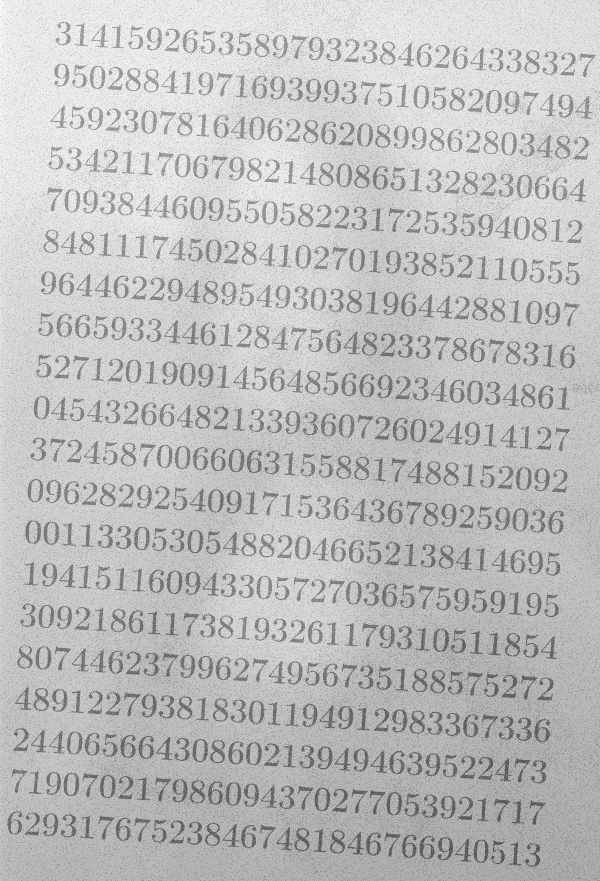
\includegraphics[scale=0.20]{data/morf_test.png}
    \caption{Imagem original}
    \label{fig1}
\end{figure}

Depois de aplicar o bottom hat e o filtro bilateral:

\begin{figure}[h]
    \centering
    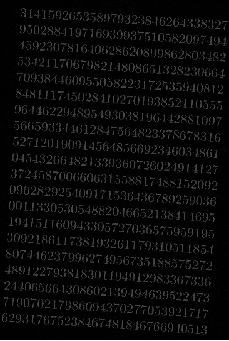
\includegraphics[scale=0.7]{data/bh1.png}
    \caption{Bottom hat aplicado}
    \label{fig2}
\end{figure}

Ao definir-se um limiar bom, converte-se a imagem para binário.

Também aplica-se o fechamento para melhorar os contornos das letras, que muitas
das vezes perdem detalhes no processos anteriores.
\begin{figure}[h]
    \centering
    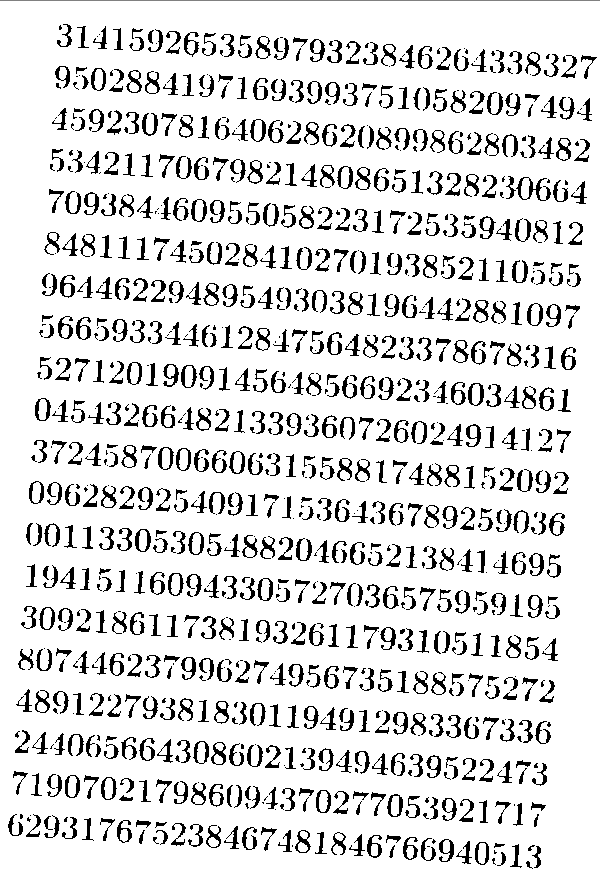
\includegraphics[scale=0.30]{data/binario1certo.png}
    \caption{Binarização}
    \label{fig3}
\end{figure}

Outro processo pedido foi a separação do fundo, fazendo fechamento chegamos ao seguinte
resultado:

\begin{figure}[h]
    \centering
    
\includegraphics[scale=0.8]{data/fundo1.png}
    \caption{Fundo separado}
    \label{fig4}
\end{figure}

\subsection{Questão 2}

A saída desse exercício é a imagem original mostrada na Imagem \ref{fig5} sem o padrão encontrado nela, 
processo feito por filtros de Butterworth.
\begin{figure}[h]
    \centering
    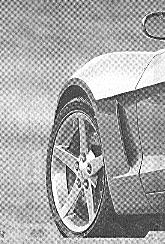
\includegraphics[scale=1]{data/moire.png}
    \caption{Image original com padrão moiré}
    \label{fig5}
\end{figure}

Pra esse processo também é encontrada a transformada de Fourier da imagem,
seu espectro de magnitude também é mostrada na Figura \ref{fig6}. 

\begin{figure}[h]
    \centering
    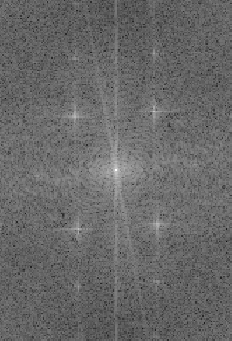
\includegraphics[scale=0.7]{data/fourier2.png}
    \caption{Espectro de magnitude}
    \label{fig6}
\end{figure}

\begin{figure}[!ht]
    \centering
    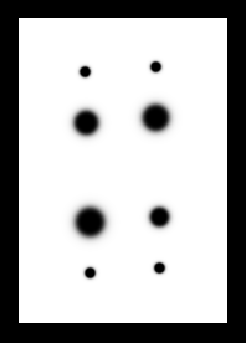
\includegraphics[scale=0.7]{data/filter2.png}
    \caption{Filtro utilizado}
    \label{fig7}
\end{figure}

Como pode-se ver na Figura \ref{fig7}, o filtro correspondente ao pedido foi encontrado e aplicado,
resultando na Figura \ref{fig8}.

\pagebreak
Abaixo, pode-se ver o resultado achado:

\begin{figure}[h]
    \centering
    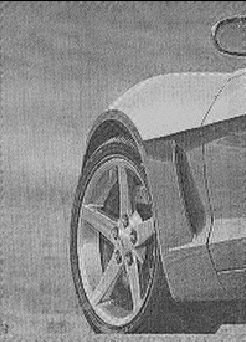
\includegraphics[scale=0.7]{data/filtered2.png}
    \caption{Imagem Moiré Filtrada}
    \label{fig8}
\end{figure}

\subsection{Questão 3}

\begin{figure}[h]
    \centering
    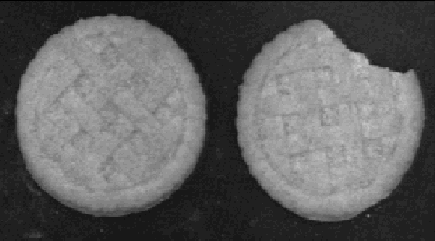
\includegraphics[scale=0.6]{data/cookies.png}
    \caption{Imagem Original dos Cookies}
    \label{fig9}
\end{figure}

A terceira tarefa era baseada em eliminar a cookie mordida, trabalhando
com transformações morfológicas.

A primeira etapa desse processo consiste na erosão da imagem deixando apenas parte
da cookie completa, isso tudo depois de binarização, como pode-se ver na Figura \ref{fig9}
\begin{figure}[h]
    \centering
    
\includegraphics[scale=0.6]{data/erode3.png}
    \caption{Cookies erodidos}
    \label{fig10}
\end{figure}

Depois disso dilata-se e se pega os pontos de interseção com o principal, chegando
ao resultado da Figura \ref{fig10}
\begin{figure}[!ht]
    \centering
    
\includegraphics[scale=0.6]{data/recover3.png}
    \caption{Cookie completa recuperada}
    \label{fig11}
\end{figure}

Em seguida, é hora de mostrar apenas a cookie completa, chegando
a saída final presente na Figura \ref{fig11}
\begin{figure}[!th]
    \centering
    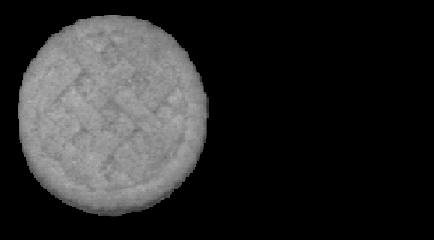
\includegraphics[scale=0.6]{data/completed3.png}
    \caption{Apenas cookie completa}
    \label{fig12}
\end{figure}

\pagebreak

\section{Conclusões}

Levando em conta toda a realização do projeto, considera-se que este foi 
executado com sucesso e com resultados aceitáveis. Apesar de ter sido concluído
de forma decente, há espaço para melhorias.

A aplicação do filtro Butterworth foi feito através de loops, se funções do Numpy
ou de outra biblioteca fossem utilizadas a velocidade de execução aumentaria consideravelmente.

Os resultados deram a perceber na prática como funcionam diversos dos conceitos
desenvolvidos em sala de aula, além de uma maior percepção do assunto.






% conference papers do not normally have an appendix






% trigger a \newpage just before the given reference
% number - used to balance the columns on the last page
% adjust value as needed - may need to be readjusted if
% the document is modified later
%\IEEEtriggeratref{8}
% The "triggered" command can be changed if desired:
%\IEEEtriggercmd{\enlargethispage{-5in}}

% references section

% can use a bibliography generated by BibTeX as a .bbl file
% BibTeX documentation can be easily obtained at:
% http://www.ctan.org/tex-archive/biblio/bibtex/contrib/doc/
% The IEEEtran BibTeX style support page is at:
% http://www.michaelshell.org/tex/ieeetran/bibtex/
%\bibliographystyle{IEEEtran}
% argument is your BibTeX string definitions and bibliography database(s)
%\bibliography{IEEEabrv,../bib/paper}
%
% <OR> manually copy in the resultant .bbl file
% set second argument of \begin to the number of references
% (used to reserve space for the reference number labels box)
\begin{thebibliography}{1}

\bibitem{OpenCV}
OpenCV Team, \emph{Open Source Computer Vision Documentation}.\hskip 1em plus
  0.5em minus 0.4em\relax opencv.org.

\bibitem{OpenCV2}
OpenCV Team, \emph{Morphological Transformations}.\hskip 1em plus
  0.5em minus 0.4em\relax Acessed in 17, May, 2019.

\bibitem{SciPy}
SciPy Team, \emph{NumPy User Guide}.\hskip 1em plus
  0.5em minus 0.4em\relax docs.scipy.org.

\bibitem{ButterworthWiki}
Wikipedia, \emph{Butterworth filter},\hskip 1em plus
  0.5em minus 0.4em\relax Acessed in 17, May, 2019.

  \bibitem{UFPR}
  Luiz Eduardo S. Oliveira, \emph{Morfologia Matemática Binária},\hskip 1em plus
  0.5em minus 0.4em\relax Processamento de imagens, www.inf.ufpr.br/lesoliveira/download/morfologia.pdf.

\end{thebibliography}




% that's all folks
\end{document}


